\documentclass[a4paper,10pt]{article}
\usepackage[utf8]{inputenc}
\usepackage[frenchkw]{algorithm2e}
\usepackage[francais]{babel}
\usepackage{graphicx}
\usepackage{amsfonts}
\usepackage{amsmath}

%opening
\title{}
\author{}

\begin{document}

\maketitle

\begin{abstract}
%a la fin
\end{abstract}

\section{Qu'est ce qu'un système de recommandation?}

\subsection{Notre approche}
Le but de notre projet est de pouvoir recommander un film ou plusieurs films à n'importe quel utilisateur. 
Pour cela, nous devons savoir à quel point un utilisateur va aimer tel ou tel film pour lui recommander (ou pas). 
Il nous faut donc une sorte d'échelle d'affinité de l'utilisateur au film : ce qui parait pertinent est alors d'estimer une note qu'un utilisateur mettrait à un film s'il le voyait.
Si cette note est au dessus d'un certain seuil, nous lui recommanderons ou bien nous recommanderons le film ayant la meilleur note prédite par exemple.
Nous voulons ainsi trouver un modèle mathématique permettant de déterminer la note que mettrait un utilisateur à un film qu'il n'a pas vu. 
Cependant il nous faut nous appuyer sur quelque chose, pour commencer à travailler il faut déjà connaître certaines informations sur des films et des utilisateurs, d'où la nécessité d'obtenir des données.

\subsection{Première difficulté : les données}
\subsubsection{Extraction des données}

Le besoin d'avoir des données nous guide vers une grande base de données appelée `` movielens '' qui est un site communautaire de recommandation de films où les utilisateurs du site notent des films de 0 à 5.
Plusieurs jeux de données y sont disponibles et diffèrent entre eux selon leur taille. 
Nous choisissons de travailler avec des notes données par 670 utilisateurs à 9125 films.
Par la suite nous nous référerons au nombres utilisateurs par $n_u$ et au nombre de films par $n_f$
Nous extrayons alors 2 fichiers : l’un contenant les $n_f$ films avec leurs titres et un numéro d'identification attribué,  
l’autre avec les notes des utilisateurs eux aussi numérotés par des identifiants.
Ce dernier fichier est un tableau avec $n_u$ lignes du type : identifiant de l’utilisateur, id du film qu’il a noté, note. 
Ces 2 fichiers étaient peu pratiques pour commencer à faire quelque chose avec,  
nous avons donc créer une fonction tableau\_des\_notes() qui permet de ranger toutes ces notes dans un tableau numpy (c koi un tableau numpy ??) nu*nf avec en lignes les utilisateurs,  
et en colonnes les films. Quand un utilisateur n’a pas vu un film donc qu’il ne l’a pas noté,  
on insère un `` Nan ''(Not a Number) qui est un `` symbole '' facile à traiter. On appellera ce tableau Y tout au long du projet. 

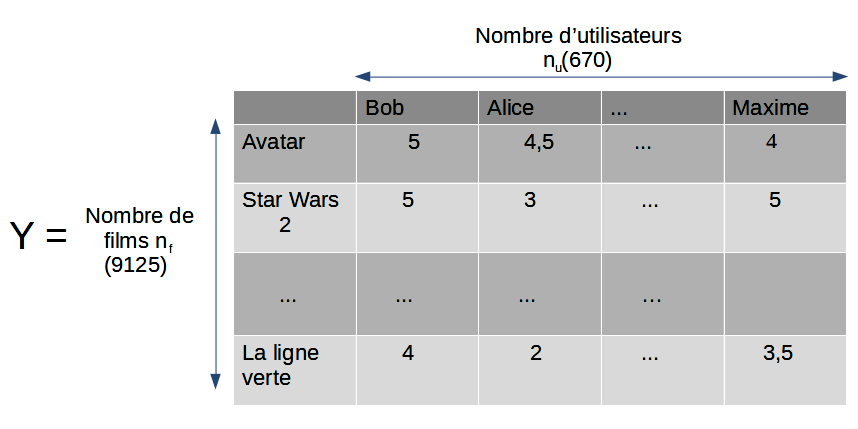
\includegraphics[scale=0.5]{matriceY.png}

\subsubsection{Analyse des données}
Dans la logique des choses, notre tableau Y étant bien trop grand pour en tirer des conclusions 
juste à l’œil, nous avons créer deux fonctions permettant de faire des sortes de statistiques sur nos données : l’une permettant de compter combien de films
chaque utilisateur a vu (cf nbre\_de\_films\_vu\_par\_utilisateur), et l’autre comptant combien de fois avait été noté chaque film 
(cf nbre\_de\_notes\_par\_film). De ces fonctions, nous avons pu tirer des graphiques nous montrant comment été répartis nos données.


Nous avons remarqué que la grande majorité des films(plus de 8000 sur 9125) possédaient entre 0 et 40 notes. 
Le nombre de notes le plus récurrents étant de 2 notes par film. Mais il y a tout de même quelques films qui ont été
beaucoup vu sachant que celui qui a le plus de note en a 339.

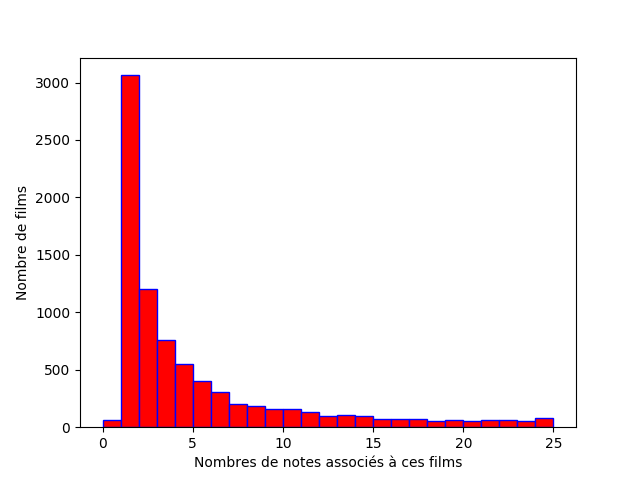
\includegraphics[scale=0.5]{hist2.png}

Dans l’autre sens,on remarque que en moyenne les utilisateurs ont noté 148 films, et la majorité (environ 550 utilisatuers sur 670) ont noté entre 0 et 250 films vus.

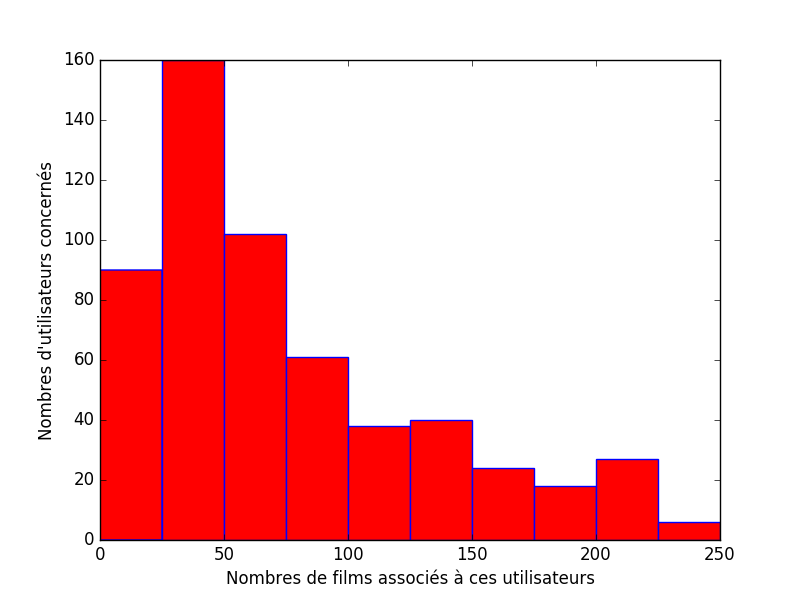
\includegraphics[scale=0.5]{hist1.png}


De plus,notre tableau présente 98,4 \% de NaN. Cela nous fait donc plus de 6 millions de notes à prédire. Dans la prochaine partie,
nous verrons donc la méthode permettant de prédire toutes ces notes à partir de très peu de données c'est à dire notre tableau Y.


\section{Formalisation du problème d'optimisation y compris modélisation}

Nous nous posons maintenant la question de comment nous y prendre pour prédire des notes ?
Notre seule ressource est la matrice Y non pleine, sur quel modèle s'appuyer pour la compléter ?
C'est ce que nous allons étudier dans cette partie.

\subsection{Quelques notations}

Introduisons quelques notations qui seront utilisées par la suite dans ce rapport.\\

Nous travaillons tout au long de ce rapport avec des matrices réelles ce qui ne sera plus précisé. $\forall (n, p) \in \mathbb{N}^2$ nous notons l'ensemble des matrices réelles de dimension $n * p$ : ${\cal M}_{n, p}$\\
$\forall (n, p) \in \mathbb{N}^2$ $\forall A \in {\cal M}_{n, p}$ $\forall i \in \{1, 2, ..., n\}$ $a_i$ est la i-ème ligne de la matrice A et nous avons $a_i \in {\cal M}_{1, p}$. Et $\forall j \in \{1, 2, ..., p\}$ $a_{., j}$ est la j-ème colonne de la matrice A et nous avons $a_j \in {\cal M}_{n, 1}$. Remarquons que des majuscules sont utilisées pour des matrices qui ne sont ni des matrices lignes ni des matrices colonnes et des minuscules autrement. Nous utilisons aussi des minuscules pour les coefficients des matrices.\\
Sauf indication contraire, lorsque nous utilisons la lettre j il s'agit d'un entier naturel non nul et inférieur ou égal à $n_f$. De la même façon la lettre i représente, lorsque ça n'est pas précisé, un entier naturel non nul et inférieur ou égal à $n_u$.\\
Enfin, le film numéro j est le film dont les notes se trouvent à la j-ème colonne de Y et l'utilisateur i est l'utilisateur dont les notes qu'il a donné sont à la i-ème ligne de Y.

\subsection{Modélisation du problème : factorisation de matrices}

Posons $Y_f$ la matrice Y complétée qui contient toutes les prédictions, exactes, des notes qui nous manquent. C'est la matrice à laquelle nous voulons aboutir, que nous devons deviner. Voici notre méthode.\\ 
 
Nous supposons que nous sommes capable de déterminer à partir de Y deux matrices X et $\Theta$ telles que $\Theta X^T = Y_f$ avec $\Theta$ une matrice de dimension $n_u * n$ et X une matrice de dimension $n_f * n$. $n \in \mathbb{N}^*$ est quelconque, nous verrons par la suite que nous pouvons le fixer comme bon nous semble.\\ 
Notre hypothèse sur l'interprétation de $\Theta$ et X ? Ce qui nous fait supposer leur existence ? Nous allons éclairer ce point tout de suite par des explications plus précises.\\

Le paragraphe qui suit est la description de nos suppositions sur l'interprétation que nous pouvons faire à propos de n, $\Theta$ et X. Après chaque verbe au conditionnel il serait possible d'ajouter "d'après notre hypothèse".\\
Parlons un peu du nombre n. Ce dernier serait en fait un nombre de caractéristiques quelconques, qui nous sont inconnues et qui peuvent bien décrire nos films : si nous pensons qu'ils peuvent être décris efficacement par 10 caractéristiques, nous choisissons de trouver $\Theta$ et X avec $n = 10$. 
Une caractéristique peut être n'importe quoi, du taux d'action au taux de blondeur des cheveux de l'actrice principale. Pour l'instant admettons seulement que ces n caractéristiques peuvent exister. Nous les numérotons de 1 à n, puis nous verrons comment elles sont déterminées dans une autre partie.\\
Décrivons X. Nous avons déjà dit que cette matrice possède $n_f$ lignes. Chaque ligne caractériserait un film. Ainsi $\forall j \in \{1, 2, ..., n_f\}$ le film j serait décrit par $x_j$ de dimension $1 * n$. Comment ? En fait $\forall k \in \{1, 2, ..., n\}$ $x_{j,k}$ correspondrait à un taux de correspondance entre le film j et la k-ième caractéristique. Si la k-ième caractéristique est l'action et si le film j est un film d'action tandis que le film j' ($j' \in \{1, 2, ..., n_f\}$) est un film romantique sans action alors $x_{j,k}$ sera un réel supérieur à $x_{j',k}$.\\
Décrivons maintenant $\Theta$. $\forall i \in \{1, 2, ..., n_u\}$ $\theta_{i}$ représenterait les goûts de l'utilisateur i. $\forall k \in \{1, 2, ..., n\}$ $\theta_{i,k}$ serait un taux d'appréciation de la caractéristique k pour l'utilisateur i.\\
Ainsi seraient les deux matrices auxquelles nous voulons aboutir.\\

Voyons maintenant voir en quoi le produit $\Theta X^T$ peut valoir $Y_f$. D'après le produit matriciel, $\forall i \in \{1, 2, ..., n_u\}$ et $\forall j \in \{1, 2, ..., n_f\}$ on a $(y_{f})_{i,j} = theta_{i}(x_{j})^{T}$ : la note que l'utilisateur i a donné ou donnera au film j dépend des caractéristiques du film et du profil de l'utilisateur. Et nous avons :
\[(y_{f})_{i,j} = \sum_{k = 1}^{n} \theta_{i,k} * x_{j,k}\]
Ce qui semble logique : la note est une combinaison linéaire des taux de caractéristiques du film avec des coefficient qui sont plus ou moins élevé suivant le goût de l'utilisateur pour la caractéristique concernée.

\subsection{Fonction de coût}

Nous avons supposé que $\Theta$ et X existent, cependant il est très peu probable que ce soit le cas : nous pouvons arriver à deux matrices avec les dimensions voulues mais avec au mieux $\Theta X^T \approx Y_f$. Notre problème devient alors la minimisation de l'écart entre les notes de $\Theta X^T$ et celles de $Y_f$. Mais nous ne connaissons que quelques notes de $Y_f$ : les notes déjà données par les utilisateurs, celles de Y. Ce qui nous amène à introduire une fonction qui estime un écart entre les notes de $\Theta X^T$ et de Y :
\begin{align*}
J\colon{\cal M}_{n_u, n} \times {\cal M}_{n_f, n} &\longrightarrow \mathbb{R}^+\\
(\Theta, X)&\longmapsto \frac{1}{2}\sum_{\substack{i,j \\ y_{i,j} \ne nan}}(\theta_{i}(x_{j})^{T}-y_{i,j})^{2}
\end{align*}
Nous appelons J fonction de coût, c'est la fonction à minimiser pour trouver $\Theta$ et X optimaux qui représentent nos données le mieux possible.

\section{Implémentation algo}
%guillaume
\subsection{descente du gradient en general optimisation}
Nous utilisons un algorithme appelé descente du gradient pour minimiser J. Pour illustrer cet algorithme nous allons l'appliquer 
à une fonction $f$ qui dépend de deux variables.%J'aimerai bien mettre la n otation pour une fonction ici
 On a $df = \frac{\partial f}{\partial x_{1}}d x_{1} + \frac{\partial f}{\partial x_{2}}dx_{2}$. En faisant l'approximation
 $\Delta f = \frac{\partial f}{\partial x_{1}}\Delta  x_{1} + \frac{\partial f}{\partial x_{2}}\Delta x_{2}$ on se rend compte
 que en posant $\Delta x_{1} = -\alpha \frac{\partial f}{\partial x_{1}}$
 et $\Delta x_{2} = -\alpha \frac{\partial f}{\partial x_{2}}$ avec $\alpha \in \Re^{+}$
 on obtient $\Delta f = -\alpha \frac{\partial f}{\partial x_{1}}^{2} - \alpha \frac{\partial f}{\partial x_{2}}^{2} < 0$. Ainsi dans
 les limites de l'approximation faite au dessus a chaque fois qu'on modifie les $x_{i}$ de $- \alpha \frac{\partial f}{\partial x_{i}}$
 on a une réduction de $f$.
On applique le même raisonnement sur $J$ avec une subtilité. Comme on arrive pas a 

\begin{algorithm}[H]
 \Donnees{this text}
 \Res{how to write algorithm with \LaTeX2e }
 initialization\;
 \Repeter{not at end of this document}{
  read current\;
  \eSi{understand}{
   go to next section\;
   current section becomes this one\;
   }{
   go back to the beginning of current section\;
  }
 }
 \caption{How to write algorithms}
\end{algorithm}
%je sais que c'est trop court et pas assez bien posé mais il faut commencer quelque part
On prouve en \ref{P1} que $ \nabla_{x_{j}}J(x, \Theta) = \nabla_{x_{j}^T}\frac{1}{2}\Vert\tilde{\theta}x_{j}^{T}-\tilde{y}_{.,j}\Vert^{2}$
puis en \ref{P2} on prouve que $[\nabla_{x} \frac{1}{2}||Ax - b||^{2}_{2}]_{j} = [A^{T}(Ax - b)]_{j}$ ce qui nous permet de dire
que $ \nabla_{x_{j}}J(x, \Theta) =  \tilde{\theta}^{T}(\tilde{\theta}x_{j}^{T}-\tilde{y}_{.,j})$. Ces divers calculs nous permettent
de représenter une étape du gradient comme une série de produits de matrices. Au début, nous devions calculer le résultat terme a terme. Cette
facon de faire était trés lente et passer à une représentation matricielle nous a permis de grandement accélerer les étapes de la descente du gradient.
\subsubsection{ecrire algo puis dire comment on a fait au début}
\section{Mise en application de l'algorithme}
\subsection{Familiarisation avec problème plus simple}
Dans la première partie de notre projet, nous avons décidé de simplifier notre problème en extrayant un tableau de données 
plein c'est à dire un tableau où tous les films ont été notés par tous les utilisateurs. 
A partir de ce tableau, nous pouvons donc enlever une note et essayer de la prédire. Ainsi, nous pouvons voir nos erreurs facilement sans avoir à gérer les Nan.
Notre première difficulté a été d'extraire ce tableau plein. Pour cela, l'étude des données faite en amont nous a beaucoup aidé: pour extraire ce tableau ``plein''
nous avons crées une fonction (cf annexe) sélectionnant les films les plus vus puis les utilisateurs qui ont vues tous ces films. On a donc obtenus un
tableau plein 10*11 (10 films pour 11 utilisateurs).
Dans ce cas-ci, nous supposons qu'il existe une relation linéaire commune pour tous les films, c'est à dire que la matrice X serait une matrice colonne.
On fixe donc tout d'abord cette matrice X aléatoirement. Puis on applique la descente du gradient pour trouver les coefficients de cette matrice les plus adaptés.
Ainsi , on peut prédire au mieux une note pour un utilisateur ayant vus tous les films d'avant.
%les trois dernière phrase sont très mal expliquer il faut les reprendre
\subsection{yassine}
\subsubsection{taux d'erreur}
Maintenant que l'on arrive à obtenir un tableau de notes rempli, c'est-à-dire dans lequel on a prédit les notes manquantes, il reste à savoir si nos prédictions sont bonnes !
Pour cela, il faut partir des choses que l'on connait : que connaissons-nous pour sûr lorsque l'on essaie de prédire des notes ? Eh bien les notes mises par des utilisateurs qui ont noté certains films.
Si notre prédiction est "efficace", on s'attend alors à ce que, si il avait fallu prédire ces notes connues, l'écart entre les notes prédites et les notes qui nous sont données aurait été faible. De but en blanc ainsi exposé, cela peut paraître flou. Mais étayons notre propos en poursuivant avec notre façon de connaître la fiabilité de notre prédiction. On l'a dit, il faudrait mesurer l'écart entre les notes prédites et les notes déjà connues. Mais comment faire en sorte que l'algorithme cherche à prédire des notes que l'on connaît déjà ? Tout simplement en lui faisant croire que nous ne les connaissons pas ! Cependant, si on efface toutes les notes connues de notre tableau de notes de départ, il est évident que l'algorithme n'aura aucune base de prédiction. C'est pourquoi nous n'effaçons qu'une partie des notes connues (10 pourcents exactement). Ainsi, on choisit 10 pourcents des notes connues de notre tableau de notes de départ (et on stocke leur emplacement dans cette grande matrice), on les transforme en NaN, puis on fournit ce nouveau tableau à l'algorithme qui nous retourne à la fin un tableau de notes plein. Ensuite, il suffit d'aller aux emplacements (que l'on a stocké au préalable) dans cette nouvelle matrice, et pour chaque note prédite à chaque emplacement, la comparer à la note connue au même emplacement (donc dans le tableau de départ). En mesurant l'écart entre chaque note, on obtient un écart moyen (le taux d'erreur) qui nous indique la fiabilité de notre prédiction : un écart peu élevé signifie que les notes prédites ont de grandes chances d'être pertinentes.
\subsubsection{influence des parametres}
Il est intéressant d'étudier les facteurs qui rendent notre prédiction plus ou moins fiable. Bien entendu, on exclue l'impact de la méthode de prédiction utilisée, celle-ci étant le choix à la base de notre projet. Nous nous demandons donc comment améliorer la fiabilité de notre prédiction sans changer complètement de méthode. Tout d'abord, le fait que l'on modélise une matrice de notes comme le produit de 2 matrices (caractérisation des films et profils des utilisateurs) implique que cette modélisation dépend du nombre de caractéristiques que l'on attribue à un film. En effet, les deux matrices étant respectivement de format (nf , nb de caractéristiques) et (nb de caractéristiques, nu), le produit de deux matrices (combinaison linéaire) implique que les coefficients du produit (les notes prédites) seront bien différentes si le nb de caractéristiques est différent. Ensuite, la descente du gradient dépend directement des "alpha" que l'on choisit. En effet, on adapte à chaque étape la matrice THETA et la matrice X en fonction d'un taux d'apprentissage alpha. En réalité, nous utilisons même 2 taux différents pour les 2 matrices. L'enjeu est de taille quant au choix de ces alphas : un trop grand alpha implique qu'en voulant se rapprocher de la note réelle, on "overshot"era, et par conséquent notre note prédite se baladera autour de la note réelle sans jamais vraiment s'en rapprocher. A l'inverse, un alpha trop petit aura pour cause des étapes du gradient qui se rapprocheraient plus du pas de fourmi qu'autre chose ... Il convient donc de trouver les alphas optimaux et le nombre de caractéristiques optimal pour obtenir de notre méthode le meilleur. A ce stade-là, vous devez sûrement vous dire que ce sont les seuls paramètres qui influent sur la précision de la méthode, mais il en est un qui est aussi essentiel. C'est le nombre d'étapes du gradient que l'on dit à l'algorithme d'effectuer. Au premier abord, notre intuition traîtreuse nous conduit à penser que plus le nombres d'étapes que l'on effectue est grand, plus grande est la précision de la prédiction. C'est en fait erroné. Certes, on se doute bien qu'une étape ou 2 ne vont pas suffir pour obtenir une note prédite pertinente, mais au bout d'un moment, il ne servira à rien de continuer à effectuer des étapes du gradient, cela desservira même notre prédiction. Nous avons observé cet effet en traçant la courbe du taux d'erreur en foncion du nombre d'étapes. Et on observe clairement un minimum du taux d'erreur pour un certain nombre d'étapes, au delà le taux d'erreur augmente. Cet effet est couramment observé en apprentissage automatique et il est surnommé "surapprentissage". Pour le contrer, nous avons donc décidé de trouver le nombre d'étapes optimal pour les alphas optimaux et le nombre de caractéristiques. optimal.
\subsection{limites de notre approche}
%yassine
\subsubsection{Est-ce qu'on arrive a reccomander un film a un utilisateur}
%guillaume
Au final une question intéressante est est-ce que le modèle arrivera d'une manière efficace a prédire les notes à un nouvel utilisateur. Pour faire cela nous avons
choisi de ne pas recalculer $X$ et $\Theta$ pour chaque nouvel utilisateur.A la place, nous supposons que l'ajout d'un utlilisateur ne va pas modifier
les caractéristiques d'un film. Il nous suffit donc de calculer $\theta$ pour l'utlisateur seulement. Ceci peut se faire trés rapidement comme notre $\Theta$ ne
consiste que du vecteur de préferences de l'utilisateur. A partir de ces nouvelles données, il nous suffit de calculer Y pour trouver la note la plus élevée et la reccomander
à l'utilisateur. Toutefois l'erreur sur la prédiction des notes nous laisse penser que ce film ne serait probablement pas le meilleur film
pour cette utilisateur ,car le hasard aurait bien pu faire que le meilleur film ait une note plus basse de 1 point ce qui suffirait à lui faire perdre la première place.
\section{Conclusion}
%1 page

\subsection{perspectives}
%guillame
\end{document}
